\newpage
\begin{minipage}{0.49\textwidth}
\section{Spannungsregler/Stromversorgung} 
\subsection{Lineare Spannungsregler\hartl{280}} 
\end{minipage}
\begin{minipage}{0.49\textwidth}
Für alle linearen Spannungsregler gilt: 
\[
P_{V}=(V_{E}-V_{a}) \cdot I_{a}
\]
\end{minipage}

\begin{longtable}{|l|l|l|}
\hline
\begin{minipage}{4cm}
\textbf{Spannungs-stabilisierung mit Transistor} \hartl{280}
\end{minipage}
&
\begin{minipage}{6cm}
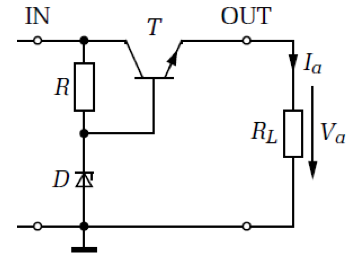
\includegraphics[width=6cm, height =
4cm]{pictures/transistorStabilisierung}
\begin{tabular}{ll}
$B$:&Gleichstromverstärkung\\[-0.8em]
$R_{i}$:&Innenwiderstand der Schaltung\\[-0.8em]
$r_{Z}$:&dyn. Innenwiderstand der Z-Diode\\[-0.8em]
$\beta$:&Stromverstärkungsfaktor des \\[-0.8em]&Transistors
\end{tabular}
\end{minipage}
&
\begin{minipage}{8cm}
\begin{gather*}
I_{E}=I_{L}\approx I_{C}\\
U_{E}=U_{A}+U_{CE}\\
U_{A}=U{Z}-U_{BE}\\
R_{V}=\frac{U_{E}-U_{Z}}{I_{Z}+I_{B}}\\
I_{B}=\frac{I_{C}}{B}\\
R_{i}\approx\frac{r_{Z}}{\beta} 
\end{gather*}
\begin{tabular}{ll}
$U_{E}$:&unstab. Eingangsspannung\\[-0.8em]
$U_{A}$:&stab. Ausgangsspannung\\[-0.8em]
$U_{Z}$:&ZDioden-Spannung\\[-0.8em]
$U_{CE}$:&Kollektor-Emitterspannung\\[-0.8em]
$U_{BE}$:&Basis-Emitterspannung\\[-0.8em]
$I_{Z}$:&Strom durch die Z-Diode\\[-0.8em]
$I_{C}$:&Kollektorstrom\\[-0.8em]
$I_{B}$:&Basisstrom\\
\end{tabular}
\end{minipage}
\\
\hline
\begin{minipage}{4cm}
\textbf{Festspannungsregler} \hartl{282}
\end{minipage}
&
\begin{minipage}{6cm}
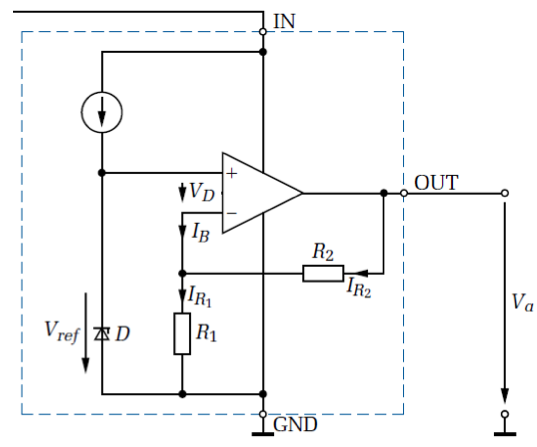
\includegraphics[height =
4cm]{pictures/festStabilisierung}
\end{minipage}
&
\begin{minipage}{8cm}
\begin{gather*}
V_{ref}=V_{D}+V_{R1}\\
V_{a}=I \cdot (R_{2}+R_{1})=\frac{V_{ref}}{r} \cdot 4R=4 \cdot V_{ref}
\end{gather*}
\end{minipage}
\\
\hline
\begin{minipage}{4cm}
\textbf{Festspannungsregler mit einstellbarer Ausgangsspannung} \hartl{284}
\end{minipage}
&
\begin{minipage}{6cm}
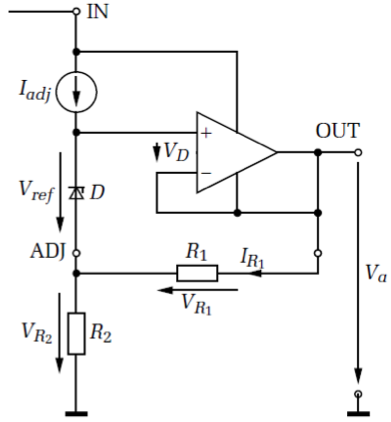
\includegraphics[height =
4cm]{pictures/einstellbarStabilisierung}
\end{minipage}
&
\begin{minipage}{8cm}
\begin{gather*}
V_{a}=V_{R1}+V_{R2}=V_{ref}+R_{2} \cdot (I_{R1}+I_{adj})=\notag\\=V_{ref}+R_{2} \cdot (\frac{V_{ref}}{R_{1}}+I_{adj})\\
\text{für }I_{adj}<< I_{R1} \to V_{a}=V_{ref} \cdot (1+\frac{R_{2}}{R_{1}})
\end{gather*}
\end{minipage}
\\
\hline
\end{longtable}


\subsection{Schaltregler\hartl{285}} 
\begin{longtable}{|l|l|l|}
\hline
\begin{minipage}{4cm}
\textbf{Ladungspumpen}
\end{minipage}
&
\begin{minipage}{6cm}
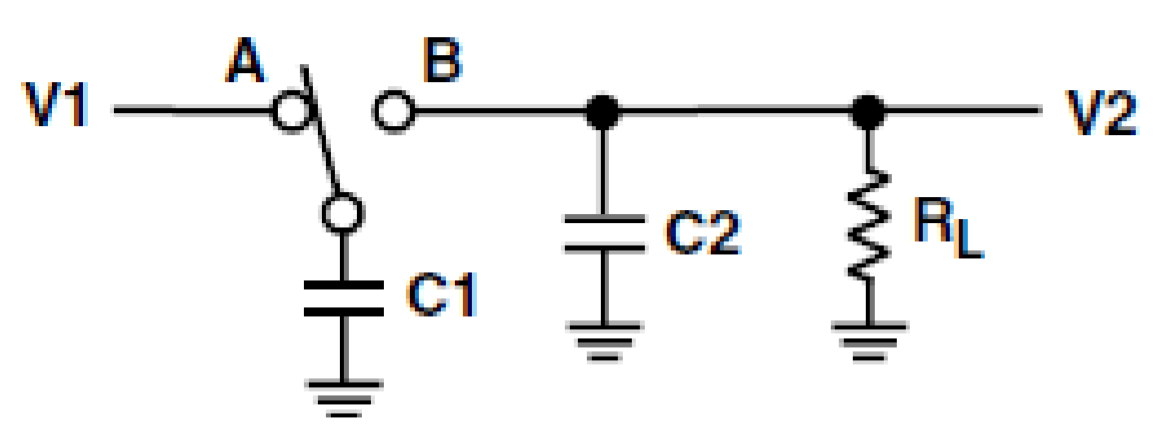
\includegraphics[width=6cm]{pictures/switchcap.png}
\end{minipage}
&
\begin{minipage}{8cm}
Rechnen über Ladungen\newline
SCPC verhalten sich gleich wie ein RC-Glied \\ $R_{eq} = \frac{1}{f_{switch}\cdot C_1} = \frac{T_{switch}}{C_1}$

Je nach dem wohin $C_1$ geschaltet wird kann die Spannung verdoppelt oder invertiert werden.

\end{minipage}
\\
\hline
\begin{minipage}{4cm}
\textbf{Abwärtswandler (Buck Converter)} \hartl{285}
\end{minipage}
&
\begin{minipage}{6cm}
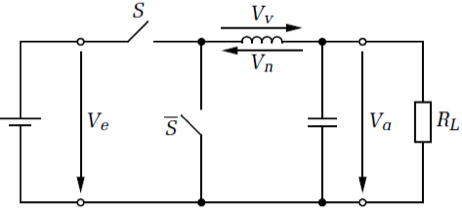
\includegraphics[width=6cm, height =4cm]{pictures/abwaertsWandler}
\end{minipage}
&
\begin{minipage}{8cm}
\begin{scriptsize}

Es gilt: $0\leq V_{a}\leq V_{e}$\\ \hrule
\begin{minipage}{0.15\textwidth}
$S_{on}$\\
\end{minipage}
\begin{minipage}{0.84\textwidth}
\begin{gather*}
V_{V}=L \cdot \frac{\Delta I_{L}}{\Delta t}\\
V_{e}=V_{V}+V_{a} \to V_{e}=L \cdot \frac{\Delta I_{L}}{\Delta t}+V_{a}\\
\end{gather*}
\end{minipage}
\hrule
\begin{minipage}{0.15\textwidth}
$S_{off}$\\
\end{minipage}
\begin{minipage}{0.84\textwidth}
\begin{gather*}
V_{n}=V_{a}=L \cdot \frac{\Delta I_{L}}{\Delta t}\\
\Delta I_{L}=(V_{e}-V_{a}) \cdot \frac{1}{L} \cdot t_{ein}\\
V_{a}=\frac{t_{ein}}{t_{aus}+t_{ein}} \cdot V_{e}=d \cdot V_{e}
\end{gather*}
\begin{tabular}{ll}
d:&Tastverhältnis/Duty Factor\\
\end{tabular}
\end{minipage}



\end{scriptsize}
\end{minipage}
\\
\hline
\begin{minipage}{4cm}
\textbf{Aufwärtswandler (Boost Converter)} \hartl{288}
\end{minipage}
&
\begin{minipage}{6cm}
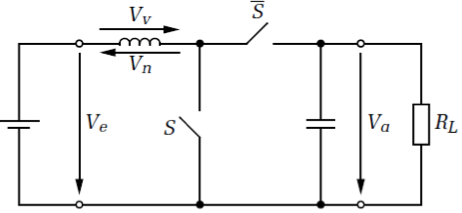
\includegraphics[width=6cm, height =4cm]{pictures/aufwaertsWandler}
\end{minipage}
&
\begin{minipage}{8cm}
\begin{scriptsize}
Es gilt : $V_{a}\geq V_{e}$\\ \hrule

\begin{minipage}{0.15\textwidth}
$S_{on}$\\
\end{minipage}
\begin{minipage}{0.84\textwidth}
\begin{gather*}
V_{v}=V_{e}=L \cdot \frac{\Delta I_{L}}{\Delta t}\\
\end{gather*}
\end{minipage}

\hrule
\begin{minipage}{0.15\textwidth}
$S_{off}$\\
\end{minipage}
\begin{minipage}{0.84\textwidth}
\begin{gather*}
V_{a}=V_{e}+V_{n}= L \cdot \frac{\Delta I_{L}}{\Delta t}+V_{e}\\
\Delta I=\frac{1}{L} \cdot V_{e} \cdot t_{ein}\\
\Delta I=\frac{1}{L} \cdot (V_{a}-V_{e}) \cdot t_{aus}\\
V_{a}=V_{e}\frac{t_{ein}+t_{aus}}{t_{aus}}=V_{e}\frac{1}{1-d}\textrm{Wenn R richtig}\notag\\\text{mit
}d=\frac{t_{ein}}{t_{aus}+t_{ein}}\\
\text{Energie im Magnetfeld:}\quad E_{L}=0.5L \cdot ipk^2
\end{gather*}
\end{minipage}
\end{scriptsize}

\end{minipage}
\\
\hline
\begin{minipage}{4cm}
\textbf{Invertierender Wandler (Buck Boost Converter)} \hartl{289}
\end{minipage}
&
\begin{minipage}{6cm}
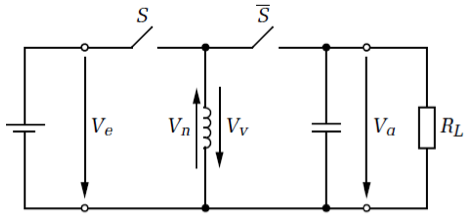
\includegraphics[width=6cm, height =4cm]{pictures/inventierenderWandler}
\end{minipage}
&
\begin{minipage}{8cm}
\begin{scriptsize}

\begin{minipage}{0.15\textwidth}
$S_{on}$\\
\end{minipage}
\begin{minipage}{0.84\textwidth}
\begin{gather*}
V_{v}=V_{e}=L \cdot \frac{\Delta I_{L}}{\Delta t}\\
\end{gather*}
\end{minipage}

\hrule
\begin{minipage}{0.15\textwidth}
$S_{off}$\\
\end{minipage}
\begin{minipage}{0.84\textwidth}
\begin{gather*}
V_{a}=-V_{n}=-L \cdot \frac{\Delta I_{L}}{\Delta t}\\
V_{a}=-V_{e} \cdot \frac{t_{ein}}{t_{aus}}=-V_{e} \cdot \frac{d}{1-d} \notag\\\text{mit
}d=\frac{t_{ein}}{t_{aus}+t_{ein}}
\end{gather*}
\end{minipage}

\end{scriptsize}

\end{minipage}
\\
\hline
\end{longtable}





\begin{minipage}{0.49\textwidth}
\subsection{Regelung der Ausgangsspannung: Voltage Mode}
\begin{itemize}
  \item Mit PWM-Signal
  \item Ist Vout zu klein, wird Ladezeit (damit Strom) erhöht $\to V_{out}$wird
  grösser
\end{itemize}

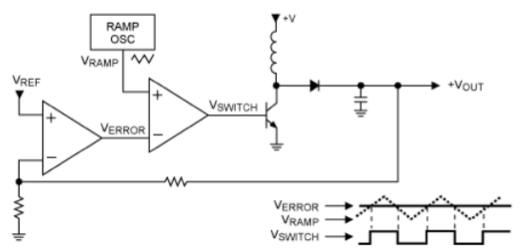
\includegraphics[width=\textwidth]{pictures/ausgangsspannungsregelung}

\end{minipage}
\begin{minipage}{0.49\textwidth}
\subsection{Regelung mit Current mode}
\begin{itemize}
  \item Strom und Spannung werden gemessen
  \item Innerer Loop muss schneller sein als äusserer Loop
\end{itemize}

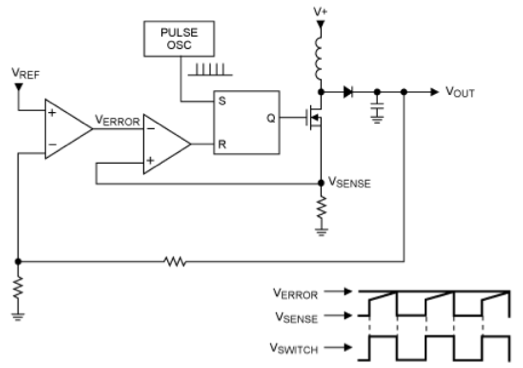
\includegraphics[width=\textwidth]{pictures/currentmode}

\end{minipage}


\subsection{Effizienzsteigerung}
\begin{minipage}{0.69\textwidth}
\subsubsection{MOSFET statt Diode}
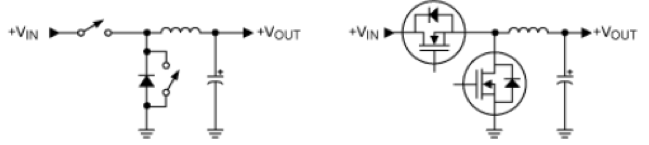
\includegraphics[scale=0.5]{pictures/effizient1}
\begin{itemize}
  \item Diode hat Spannungsabfall
  \begin{itemize}
    \item Silizium-Diode: 0.7V
    \item Schottky-Diode: 0.3V
    \item MOSFET hat "`nur"' On-Widerstand $Rds_{on}$
    \end{itemize}
   \item Umschalten vom Substratpotential beim Längstransistor nötig
   \begin{itemize}
     \item Synchronous rectifier
    \end{itemize}
\end{itemize}
\end{minipage}
\begin{minipage}{0.29\textwidth}
\subsubsection{Skip-Mode}
\begin{itemize}
  \item Lade- und Entladezyklen werden ausgelassen bei niedrigem Laststrom
\end{itemize}
\end{minipage}


%\begin{figure}[h!]
%
%	\centering
%	\begin{subfigure}[b]{0.45\textwidth}
%		\centering
%		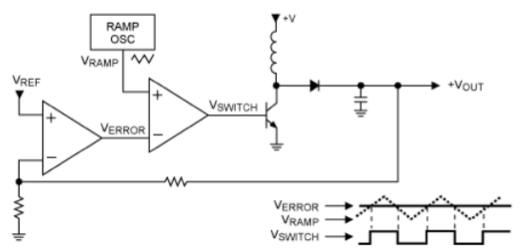
\includegraphics[width=\textwidth]{pictures/ausgangsspannungsregelung}
%		\caption{Voltage Mode}
%	\end{subfigure}
%	\qquad
%	\begin{subfigure}[b]{0.45\textwidth}
%		\centering
%		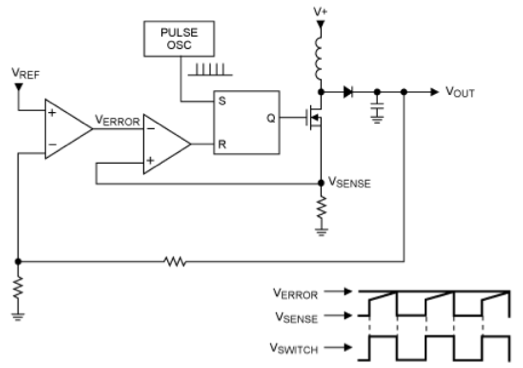
\includegraphics[width=\textwidth]{pictures/currentmode}
%		\caption{Current Mode}
%	\end{subfigure}
%	\caption{Vergleich Current Mode / Voltage Mode}
%\end{figure}
%
%
%\newpage
%\subsection{Effizienzsteigerung}
%\subsubsection{MOSFET statt Diode}
%\begin{figure}[htb]
%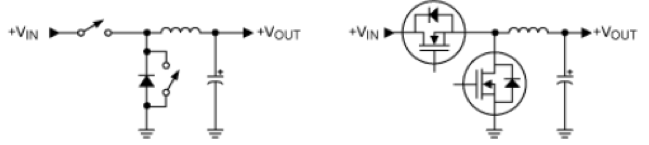
\includegraphics[scale=0.5]{pictures/effizient1}
%\end{figure}
%\begin{itemize}
%  \item Diode hat Spannungsabfall
%  \begin{itemize}
%    \item Silizium-Diode: 0.7V
%    \item Schottky-Diode: 0.3V
%    \item MOSFET hat "`nur"' On-Widerstand $Rds_{on}$
%    \end{itemize}
%   \item Umschalten vom Substratpotential beim Längstransistor nötig
%   \begin{itemize}
%     \item Synchronous rectifier
%    \end{itemize}
%\end{itemize}
%
%\subsubsection{Skip-Mode}
%\begin{itemize}
%  \item Lade- und Entladezyklen werden ausgelassen bei niedrigem Laststrom
%\end{itemize}
